\documentclass[12pt]{ctexart}
\usepackage{amsmath, amssymb}
\usepackage{graphicx}
\usepackage{booktabs}
\usepackage{hyperref}
\usepackage{geometry}
\usepackage{mathrsfs}
\usepackage{tcolorbox}
\usepackage{float}
\usepackage{hyperref}
\usepackage{tabularx}
\usepackage{booktabs}
\geometry{a4paper, margin=2.5cm}
\renewcommand{\tabularxcolumn}[1]{m{#1}}


\setCJKmainfont[
    BoldFont=Noto Serif CJK TC Bold,
    ItalicFont=Noto Serif CJK TC
]{Noto Serif CJK TC}

\title{運用集成式學習預測台灣珊瑚礁的覆蓋面積}
\author{TRex}
\date{February 2026}

\begin{document}

\maketitle

\section{前言}
此資料為運用集成式學習預測台灣珊瑚礁的覆蓋面積中的研究過程，此研究是順著本人高中所做過的《利用機器學習預測珊瑚礁面積》的小論文往下延伸。修補了小論文中的瑕疵，並使用了更複雜的模型及工程。

\subsubsection{研究動機}
珊瑚礁作為海洋生態環境的重要生存指標，但 30 年來，氣候變化導致超過半數的珊瑚礁生態系統的死亡，卻幾乎沒有做任何事情來拯救。1998 年，全球有整整16\%的熱帶珊瑚礁死亡，而到了 2016 年，情況變得更糟了：全球 70\%的珊瑚礁遭到破壞，有些更是無法挽回的。這一年，澳大利亞的大堡礁有整整 30\%的珊瑚礁慘遭浩劫，而更糟的是，在隔年夏天，這個數據上升到了 50\%。（Ruth Gates，2016）。而指標性生物常用於測量環境品質，反推區域受到污染的情形，本研究希望透過觀察指標性生物的族群變化來進行生物監測，因此本研究將整合台灣各海域的指標性生物的數據透過機器學習去預測珊瑚礁的覆蓋率。

\subsubsection{研究目的}

\begin{enumerate}
    \item 透過集成式學習比較四種不同的機器學習方法在預測台灣珊瑚礁覆蓋率上的效力
    \item 了解各指標性生物與珊瑚間重要性、找出最有影響力的特徵並架構關係圖
    \item 為珊瑚礁的現況提供解方以及可努力的方向。
\end{enumerate}

\section{文獻探討}

\subsection{珊瑚礁概況}
2022 年 6 月，台灣環境資訊協會公布了台灣珊瑚礁體檢 12 年的成果報告，從 2009 年到 2020 年，內容包含台灣和離島的珊瑚礁海域，一共 25 處珊瑚礁生態的長期變化。報告中，以「生態健康紅綠燈」的燈號顯示，說明各地珊瑚礁生態系的總體健康程度。其中「紅燈」代表健康岌岌可危，共有三處，為北海岸與東北角、東海岸、小琉球。「黃燈」代表健康堪憂，也有三處，為墾丁、綠島、澎湖嶼坪。「綠燈」代表健康良好，但只有蘭嶼是綠燈 (台灣資訊協會，2020)

\subsection{指標性生物}
國際社會目前大多採用「物種指標」來表示生物多樣性變化， 而物種指標需要具備下列特徵(The Work Banks，1995 )：具有足夠的敏感性來指示早期的環境變化，它具有環境變遷的預警作用、具有較廣的地理分布範圍、當環境改變時，此類生物的分布範圍也會改變，而容易被偵測出來、比較容易收集資料及量度者、能夠用來反應只是因人類干擾而產生的變化。而台灣資訊協會（2019）對珊瑚的指標性生物評選標準與國際社會的標準相符，因此台灣資訊協會的數據具有參考價值。

\section{研究方法}
描述原資料集中的資料以及如何透過其他技術去獲得對模型有幫助之資料。

\subsection{研究樣本}

「台灣資訊協會」自 2008 年起展開「台灣珊瑚體檢」志工行動計劃，調查台灣7個地區的活珊瑚覆蓋率及指標生物數量，並探討環境對珊瑚礁的影響（台灣資訊協會，2022），其中 6 個地區檢測頻率為年資料，而墾丁則因為調查較晚所以檢測頻率為半年一次。調查地區分別為潘仔澳、基翬、墾丁、母雞岩、玉女岩、東嶼西側、東嶼東側、東嶼南側，而資料共分為「底質類群」、「環境衝擊」、「指標性魚類」、「指標性底棲無脊椎動物」四類。（如表1）

\begin{table}[H]
    \centering
    \caption{所有特徵}
    \vspace{2mm}
    \begin{tabularx}{\textwidth}{|l|X|}
        \hline
        \textbf{特徵類別} & \textbf{特徵} \\ \hline
        底質類群 & 硬珊瑚、軟珊瑚、新死珊瑚、營養鹽指標性藻類、海綿、岩石、碎石、細沙、泥沙、其他 \\ \hline
        環境衝擊 & 重物敲擊造成之珊瑚損害、爆裂物造成之珊瑚損害、其他原因造成之珊瑚損害、漁業垃圾、一般垃圾 \\ \hline
        指標性魚類 & 石鱸、笛鯛、石斑、裸胸鯙、蘇眉、蝴蝶魚、鸚哥魚、隆頭鸚哥 \\ \hline
        指標性底棲無脊椎動物 & 大法螺、魔鬼海膽、馬糞海膽、鉛筆海膽、棘冠海星、龍蝦、櫻花蝦、梅花參、硨磲貝 \\ \hline
    \end{tabularx}
\end{table}

為了檢視生物與珊瑚之關係，指標性生物的食性是十分重要的，其食群可分為「食肉性」、「食藻性」、「食珊瑚性」、「食屑性」、「其他」五大類。（如表2）

\begin{table}[H]
    \centering
    \caption{指標性生物食性表}
    \vspace{2mm}
    \begin{tabularx}{\textwidth}{|l|X|}
        \hline
        \multicolumn{1}{|c|}{\textbf{食性}} & \multicolumn{1}{c|}{\textbf{生物}} \\ \hline
        食肉性 & 石鱸、笛鯛、石斑、老鼠魚、裸胸鯙、蘇眉、大法螺 \\ \hline
        食藻性 & 魔鬼海膽、馬糞海膽、鉛筆海膽 \\ \hline
        食珊瑚性 & 蝴蝶魚、鸚哥魚、隆頭鸚哥、棘冠海星 \\ \hline
        食屑性 & 龍蝦、櫻花蝦、梅花參 \\ \hline
        其他 & 硨磲貝 \\ \hline
        \multicolumn{2}{|l|}{註：台灣資訊協會於 2019 年整理} \\ \hline
    \end{tabularx}
\end{table}

\subsection{資料擴增}
由於原始的資料中只包含各種生物、測量地點以及一些危害的特徵，缺乏會直觀影響珊瑚礁的環境因子，如當地的洋流、氣溫、降水量等，因此在原始資料外又加入了三項特徵，「測量地點的經緯度」、「前30日平均氣溫」以及「前30日降水量」。

\subsubsection{測量地點的經緯度}
測量地點的經緯度在另一份由協會提供的資料中亦存在，其中包含了8個地點的經緯度準確至小數點後兩位。由此資料即可判斷此地點位於台灣的東海岸、西海岸抑或是離島。

\begin{figure}[H]
    \centering
    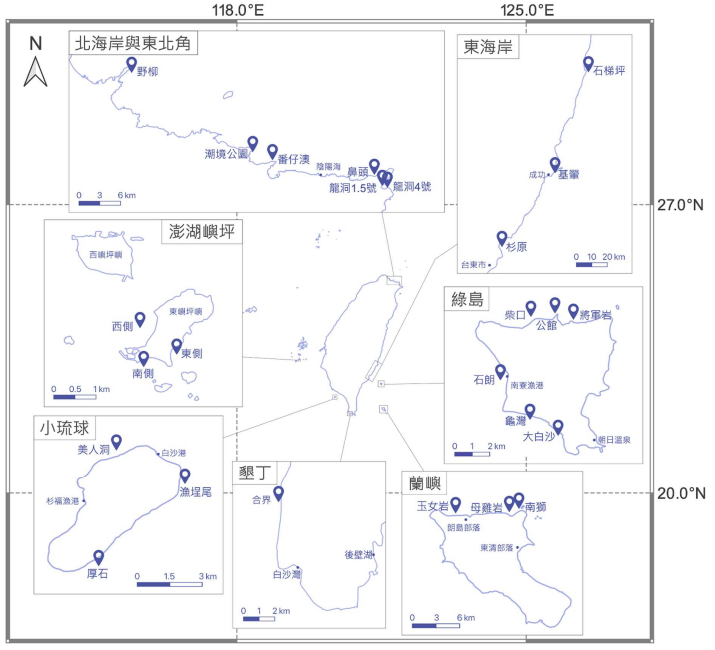
\includegraphics[width=0.6\linewidth]{珊瑚礁體檢地點.png}
    \caption{珊瑚礁體檢地圖(節錄自台灣珊瑚礁體檢 12 年成果報告(2009~2020)第㇐版)}
    \label{fig:placeholder}
\end{figure}

\subsubsection{氣象資料}
Python Open-Meteo API 是一個免費、開源且無需註冊 API 金鑰的天氣數據服務，只需要提供欲查詢地點的經緯度以及時間即可獲得當時的天氣資料。利用此做法查詢6個觀測區域內每個觀測點觀測時間前三十天的平均氣溫與平均降雨量以及前三個月的累積熱壓力(accumulated heat stress)

\subsubsection{時間序列}
由於此資料為時間序列資料，因此捕捉目標資料的時間趨勢是十分重要的，因此使用了滯後特徵(Lag feature)，將前一次的珊瑚礁覆蓋面積納入特徵，同時也使用 Meta 的 Prophet 抓取序列趨勢，兩者一起使用的情況下獲得了更顯著的結果。

\subsubsection{訓練資料}
本次研究希望探討各生物對珊瑚礁的影響，故變數如下：
\begin{table}[H]
    \centering
    \caption{變數表}
    \vspace{2mm}
    \begin{tabularx}{\textwidth}{|l|X|}
        \hline
        \multicolumn{1}{|c|}{\textbf{變數}} & \multicolumn{1}{c|}{\textbf{特徵}} \\ \hline
        目標變數 & Coral\_Cover \\ \hline
        訓練變數 & NIA, SP, Butterflyfish, Haemulidae, Snapper, BarramundiCod, HumpheadWrasse, BumpheadParrotfish, Parrotfish, MoralEel, Grouper\_XS, Grouper\_S, Grouper\_M, Grouper\_L, Total\_fish, BandedCoralShrimp, Diadema, PencilUrchin, CollectorUrchin, SeaCucumber, COTS, Triton, Lobster, GiantClam\_XS, GiantClam\_S, GiantClam\_M, GiantClam\_L, GiantClam\_XL, GiantClam\_XXL, Coast, Avg\_Temp\_30d, Total\_Rain\_30d, Lag\_Coral\_Cover,	prophet\_pred, accumulated\_heat\_stress \\ \hline
        其他變數 & Date, Site, Date, lat, lon \\ \hline
    \end{tabularx}
\end{table}
目標變數包含了硬珊瑚(HC)、軟珊瑚(SC)以及新死珊瑚(RKC)的資料，而訓練變數內則是大部分的生物變數再加上地點、前三十天平均氣溫以及前三十天平均雨量。而總共有1332筆資料，為了避免隨機抽取造成滯後特徵和 Prophet 不小心做到預知未來的能力，資料集是以時間作為劃分。將資料按照 "Date" 排序，再讓前 $80\%$ 的資料用於訓練，剩下的 $20\%$ 用於預測。

\subsection{研究模型}
本次研究使用了三個在Kaggle上對付tabular資料無往不利的三個模型XGBoost、LightGBM、CatBoost以及由Google團隊研發，號稱能完勝前三者的神經網路模型TabNet，這四個模型不只強大還保留了一定的解釋力，對了解指標性生物對珊瑚礁的影響具有十分的幫助。

\subsubsection{TabNet}
TabNet身為深度學習模型，對於特徵間的關聯性有著強大的捕捉能力，使得能在沒有太多特徵工程的情況下一樣可以有很好的表現，但前提是在資料量足夠龐大的情況下。本次研究雖然有12年的資料，但基於都是人工採集，故只有1100筆資料可供模型訓練。因此使用自監督預訓練 (Self-supervised Pre-training)遮蓋 $80\%$ 的資料，讓其先自行捕捉內部的趨勢，調整的參數如下：

\[
\begin{cases}
    max \ epochs=100 \\
    patience=10 \\
    batch \ size=128 \\
    virtual \ batch \ size=16 \\
    pretraining \ ratio=0.8
\end{cases}
\]

接著使用 Grid Search 來尋找參數間的最佳解，其中 $cv=3$ 且 scoring=neg\_mean\_absolute\_error，調整的參數如下：

\[
\begin{cases}
    n_d: [4, 8] \\
    n_a: [4, 8] \\
    n_steps: [2, 3] \\
    gamma: [1.3, 1.5] \\
    lambda_{sparse}: [1e-1, 1e-2] \\
    momentum: [0.02, 0.05] \\
    n_{shared}: [2] \\
    n_{independent}: [2] \\    
\end{cases}
\]

最後模型的訓練參數如下：

\[
\begin{cases}
    max \ epochs=100 \\
    patience=10 \\
    batch \ size=128 \\
    virtual \ batch \ size=16 \\
\end{cases}
\]

其中由於訓練資料較小，不論是擬合時的資料抑或是預訓練的資料都往此方向去調整。

\subsubsection{XGBoost}
作為 tabulat data 中的常態佼佼者，其本身就具備著能夠直接處理時間序列資料的能力，而在參數調整下一樣是使用Grid Search，調整的參數如下：

\[
\begin{cases}
    n_{estimators}: [100, 300] \\
    learning \ rate: [0.01, 0.1] \\
    max \ depth: [3, 7] \\
    subsample: [0.8, 0.9] \\
    reg_{alpha}: [0, 0.1] \\
    reg_{lambda}: [0, 1] \\
    min \ child \ weight: [3, 5]
\end{cases}
\]

其中由於訓練資料較小，大部分的參數都往符合此趨勢的情況去調整。

\subsubsection{CatBoost}

CatBoost 是一種基於梯度提升決策樹的機器學習演算法，一樣使用Grid Search進行Hyperparameter Tuning，其中的參數為：

\[
\begin{cases}
    iterations: [200, 500] \\
    learning \ rate: [0.03, 0.1] \\
    depth: [4, 6] \\
    random \ strength: [1, 2]
\end{cases}
\]

其中由於訓練資料太少，迭代次數、學習率以及其他變數都往符合此趨勢的情況去調整。bootstrap type 的型態為 MVS，CV = 3。

\subsubsection{LightGBM}

LightGBM 的核心特點是速度極快且記憶體佔用低，其中一樣使用Grid Search進行參數調整，其中參數如下：

\[
\begin{cases}
    n_{estimators}: [100, 300] \\
    learning \ rate: [0.05, 0.1] \\
    num_{leaves}: [7, 15] \\
    feature \ fraction: [0.7, 0.8] \\
    bagging \ fraction: [0.7, 0.8] \\
    boosting \ type: ['gbdt', 'dart'] \\    
\end{cases}
\]

其中由於訓練資料太少，選擇了較淺的樹和較少的子葉數量，且使用了bagging fraction 與 feature fraction，讓模型不要過度專注於某些資料。

\subsubsection{Meta-Learner}
將上述四個模型的預測結果輸出，並將其視為四種特徵資料去進行線性擬和，達到為每個模型提供權重的功能，並將其結果作為最後的結果。

\section{研究結果}

\subsection{模型結果}
四個模型與最後的集成式模型的結果如下：

\begin{table}[H]
    \centering
    \caption{模型結果}
    \vspace{2mm}
    \begin{tabularx}{\textwidth}{|l|X|X|X|}
        \hline
        \multicolumn{1}{|c|}{\textbf{模型}} & \multicolumn{1}{c|}{\textbf{MAE}} & \multicolumn{1}{c|}{\textbf{MSE}} & \multicolumn{1}{c|}{\textbf{R-square}} \\ \hline
        TabNet   & 0.1002 & 0.0150 & 0.7157 \\ \hline
        XGBoost  & 0.0962 & 0.0140 & 0.7358 \\ \hline
        CatBoost & 0.0924 & 0.0132 & 0.7507 \\ \hline
        LightGBM & 0.0924 & 0.0129 & 0.7550 \\ \hline
        Meta-Learner & 0.0893 & 0.0124 & 0.7653 \\ \hline
    \end{tabularx}
\end{table}

可以看到各個模型中，Meta-Learner 表現最好、再者是 LightGBM、其後是 CatBoost 與 XGBoost，最後才是 TabNet。

但在Meta-Leaner的擬和中可以發現(如圖2)，LightGBM 是權重最高者，其次是 TabNet 與 CatBoost，而 XGBoost 卻變成了負的權重。

\begin{figure}[H]
    \centering
    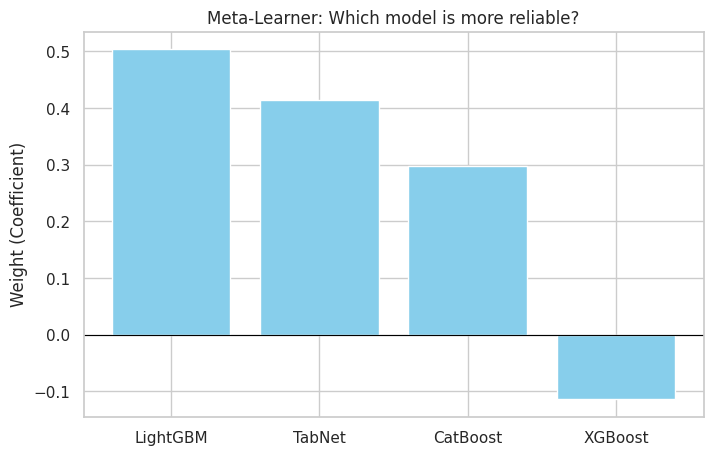
\includegraphics[width=0.75\linewidth]{Meta-Learner中的各模型表現.png}
    \caption{Meta-Learning中各模型的表現}
    \label{fig:placeholder}
\end{figure}

\subsection{各模型中的特徵重要性}
各模型中最重要的前15名特徵的結果如下圖3。
\begin{figure}[H]
    \centering
    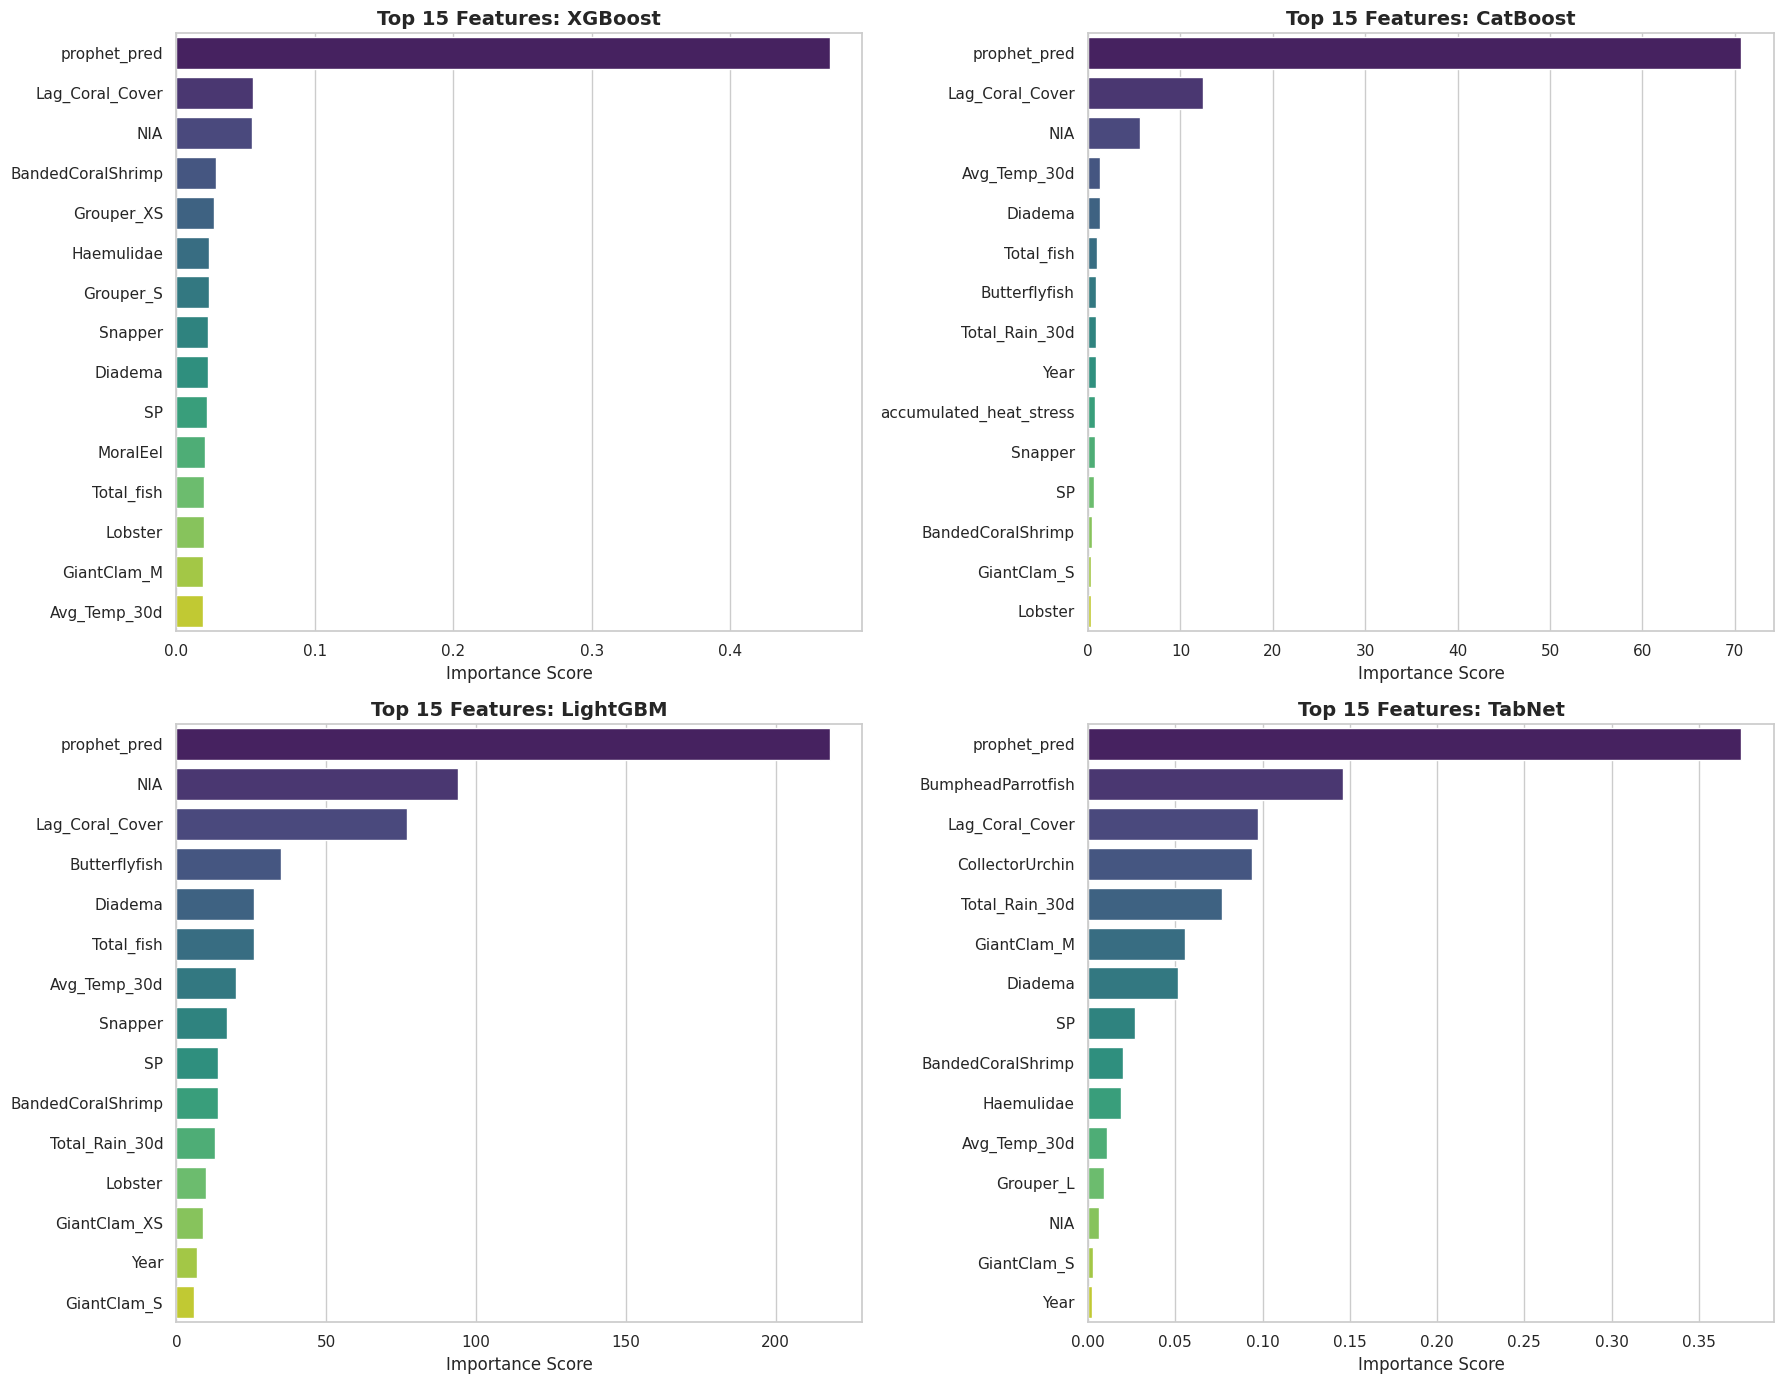
\includegraphics[width=0.75\linewidth]{各模型中最重要的前15名特徵.png}
    \caption{各模型中最重要的前15名特徵}
    \label{fig:placeholder}
\end{figure}

可以看到，不論何者模型 prophet\_pred 都是非常重要的特徵，但 XGBoost 和 CatBoost 這兩個模型中都過於依賴此特徵，這也導致雖然在一開始單獨有著較為優秀的預測結果，但在後面的集成式模型中獲得了較低的權重。而LightGBM 與 TabNet 有更偏重於各種不同的特徵，雖然 prophet\_pred 一樣有最高的重要性，但其他特徵的重要性有顯著提升。

整理完後重要的特徵如下：NIA, SP, Butterflyfish, BumpheadParrotfish, Total\_fish, BandedCoralShrimp, Diadema, Lobster, GiantClam\_XS, Avg\_Temp\_30d, Total\_Rain\_30d, Lag\_Coral\_Cover,	prophet\_pred。就生物類別的資料而言，對珊瑚礁有影響的特徵與其可能原因如下表5：
\begin{table}[H]
    \centering
    \caption{重要的生物相關特徵}
    \vspace{2mm}
    \begin{tabularx}{\textwidth}{|l|X|}
        \hline
        \multicolumn{1}{|c|}{\textbf{特徵}} & \multicolumn{1}{c|}{\textbf{原因}}  \\ \hline
        NIA & 底質藻類會直接與珊瑚礁競爭生存空間，且附著在珊瑚礁上 \\ \hline
        SP & 居住在海床的海綿也會直接與珊瑚礁競爭生存空間 \\ \hline
        Butterflyfish   & 多數蝴蝶魚以珊瑚蟲為食，且本身數量較多，樣本數足夠 \\ \hline
        Bumphead Parrotfish  & 大型草食性魚類，會啃食珊瑚礁上的海藻。 \\ \hline
        Total\_fish & 高總魚量意味著食物網結構完整，較能緩衝環境壓力。 \\ \hline
        Banded Coral Shrimp & 能移除魚類身上的寄生蟲，間接影響到珊瑚礁 \\ \hline
        Diadema & 草食性無脊椎動物，太少會使珊瑚礁過度被藻類覆蓋，過多又會磨損其骨架 \\ \hline
        Giant Clam\_XS & 小硨磲貝可以淨化水質，保養環境 \\ \hline
    \end{tabularx}
\end{table}

由表五建製的生物關係圖如下圖4：
\begin{figure}[H]
    \centering
    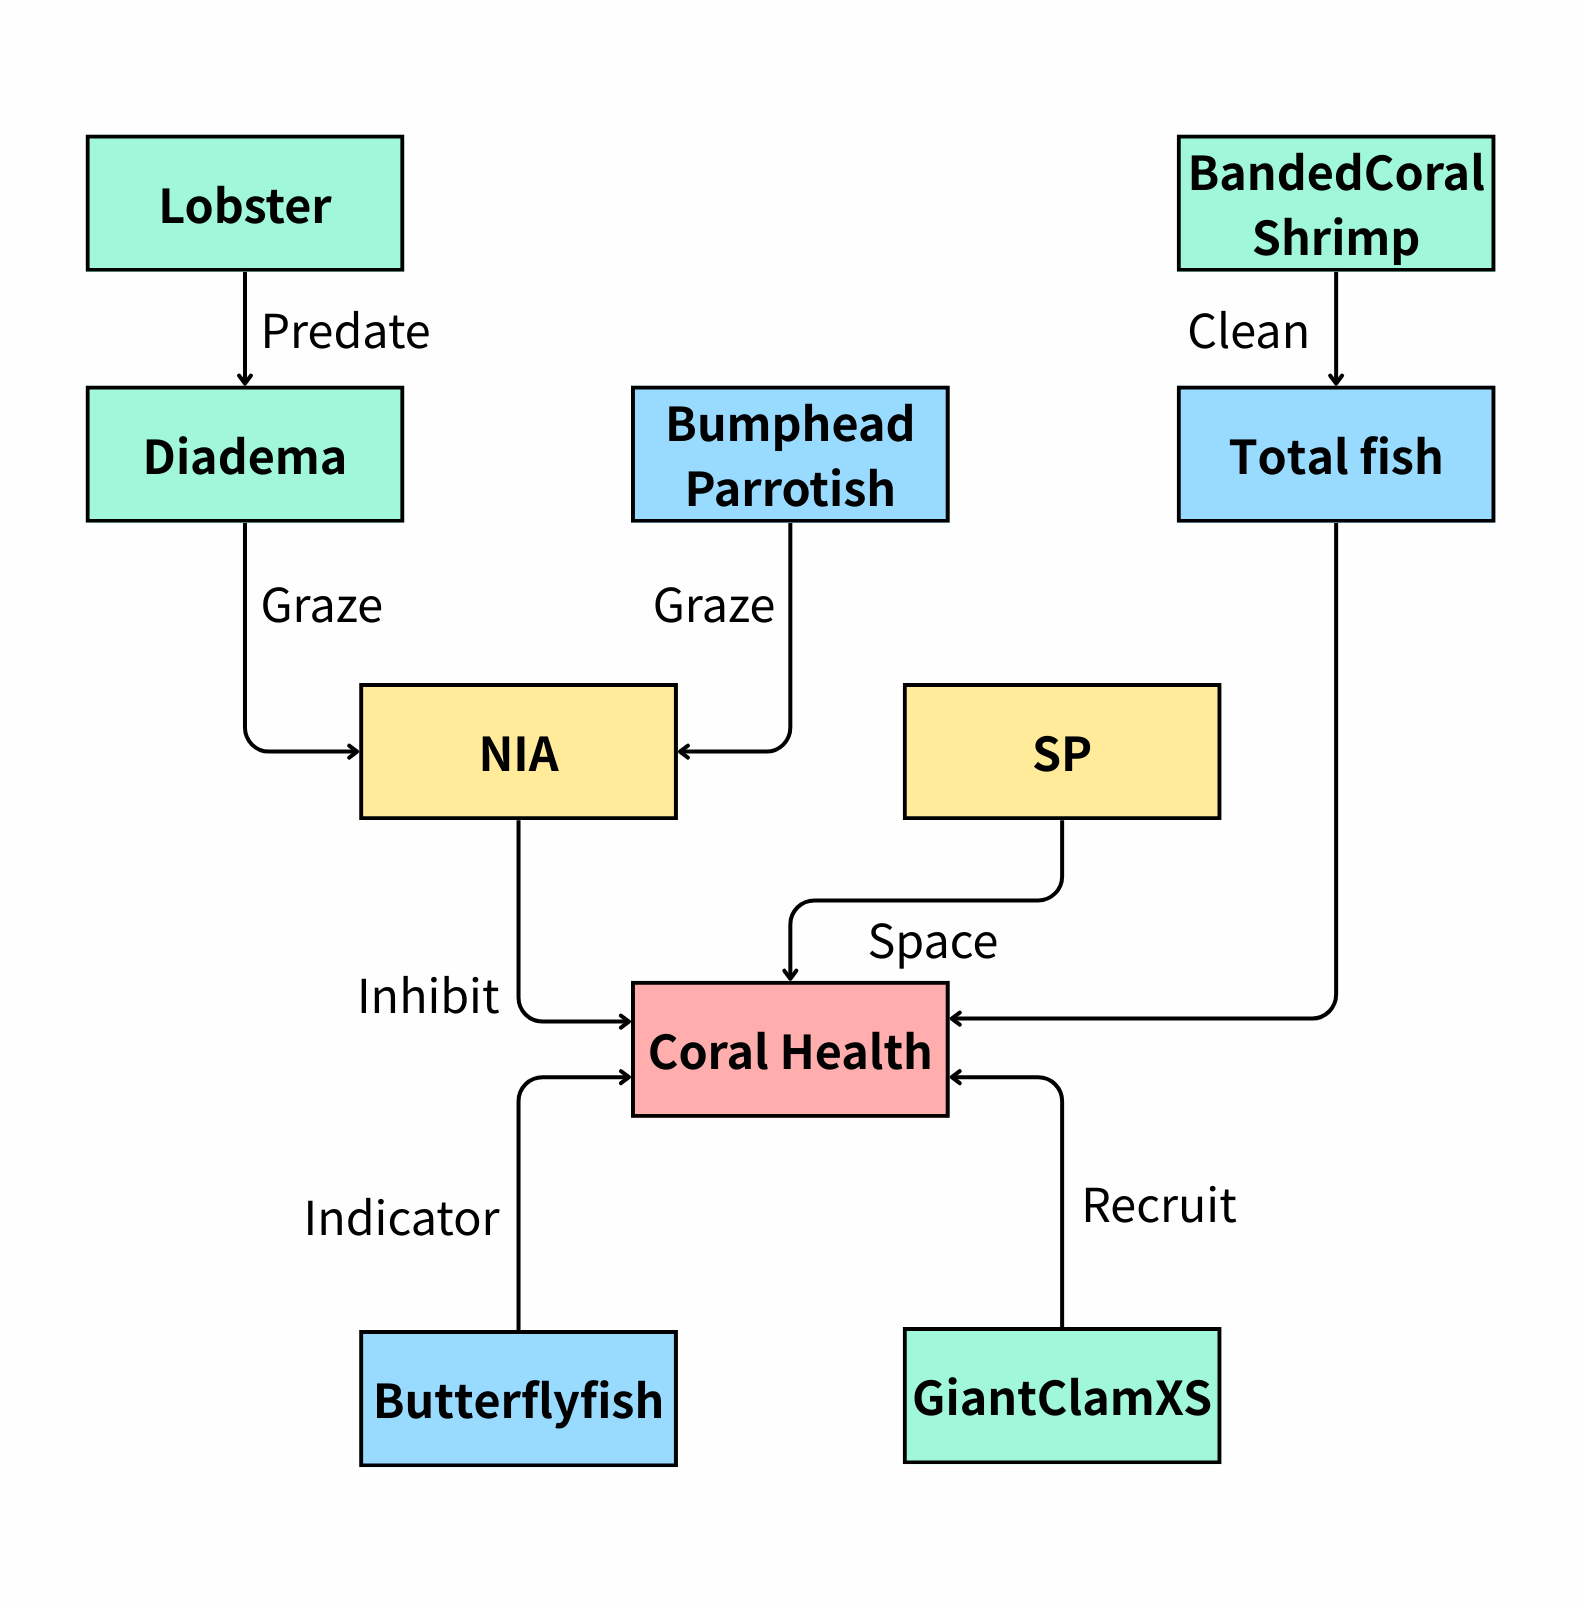
\includegraphics[width=0.6\linewidth]{生物關係圖.png}
    \caption{生物關係圖}
    \label{fig:placeholder}
\end{figure}

\section{研究討論與建議}
\subsection{結論}
\begin{enumerate}
    \item 雖然TabNet是被開發來在Tabular Data領域超越過往的主流模型的，但在資料集較少的情況下，仍心有餘而力不足。
    \item TabNet以及LightGBM能夠確實的在複雜的特徵環境中捕捉到各項指標生物的影響，這也印證了其可以避免過度專注的功能。
    \item 由最後的特徵重要性可知，本次研究中與珊瑚覆蓋面積相關生物為： NIA, SP, Butterflyfish, Bumphead Parrotfish, Total\_fish, Banded Coral Shrimp, Diadema, Giant Clam\_XS，透過關係圖亦可以知道這些特徵皆與珊瑚礁的覆蓋面積有著直接或是一次性間接的關係。
\end{enumerate}
\subsection{未來展望}
在台灣資訊協會的調查下，大部分指標性生物的數值皆不高，使得理論上能影響珊瑚礁的生物，卻對模型沒有任何助益，例如：棘冠海星（COTS）為珊瑚礁的天敵，在澳洲大堡礁對珊瑚礁影響甚大，在台灣海域卻基本上沒數據，因此後續研究將以收集全球各地的珊瑚礁覆蓋率及指標性生物作為研究方向。

此外，台灣資訊協會在每一個測試點的資料量也過於稀少，使得時間序列模型在趨勢的捕捉上沒有到十分精準，因此仍然可以期待未來，台灣資訊協會採集到更多資料後的結果。

\section{參考資料}

\begin{enumerate}
    \item 鄭楊蓁（2022）使用機器學習預測股市趨勢-台灣上市公司為例。國立雲林科技大學財務金融系：碩士論文。
    \item 魏佳美（2018）運用資料探勘預測旅遊需求。國立交通大學管理學院：碩士論文。
    \item 王禎祥（2021）應用機器學習回歸模型於成衣製造業銷售預測以 T 公司為例。國立中央大學資訊管理學系：碩士論文。
    \item 林明瑞、巫麗雯、劉惠元（2008）校園生物棲地物種指標建構之研究。台中教育大學報 22期 p 59-82
    \item 吳易樺、黃朝熙、劉子衙（2014）時間序列模型對我國產業成長預測之優劣比較。應用經濟論叢 96 期 p 35-68。
    \item 楊明錞、黃英傑、梨煥玄（2011）運用灰色馬可夫鍊預測 7-ELENEn 的營收。明新學報第 38 卷 第 1 期 p 147-161。
    \item 台灣資訊協會（2022）台灣珊瑚礁體檢 12 年成果報告。
    \item 海洋委員會海洋保護署（2022）珊瑚礁生態系。 \\ https://www.oca.gov.tw/ch/home.jsp?id=176&parentpath=0,5,173
    \item 國立自然博物館（2011）什麼是刺絲胞動物？ \\ http://digimuse.nmns.edu.tw/da/collections/az/cn/
    \item Zoe Cormier（2019 年 4 月 11 日）Saving Coral。BBC NEWS \\ https://www.bbc.com/ukchina/trad/vert-earth-47890492
\end{enumerate}


\begin{tcolorbox}
筆記作者：TRex \\ 
\end{tcolorbox}

\end{document} 
